\section{Einleitung}
Sed ut perspiciatis unde omnis iste natus error sit voluptatem accusantium doloremque laudantium, totam rem aperiam, eaque ipsa quae ab illo inventore veritatis et quasi architecto beatae vitae dicta sunt explicabo. Nemo enim ipsam voluptatem quia voluptas sit aspernatur aut odit aut fugit, sed quia consequuntur magni dolores eos qui ratione voluptatem sequi nesciunt. Neque porro quisquam est, qui dolorem ipsum quia dolor sit amet, consectetur, adipisci velit, sed quia non numquam eius modi tempora incidunt ut labore et dolore magnam aliquam quaerat voluptatem.\footcite[Vgl.][]{testOnline} Ut enim ad minima veniam, quis nostrum exercitationem ullam corporis suscipit laboriosam, nisi ut aliquid ex ea commodi consequatur? Quis autem vel eum iure reprehenderit qui in ea voluptate velit esse quam nihil molestiae consequatur, vel illum qui dolorem eum fugiat quo voluptas nulla pariatur?\footcite[Vgl.][S. 83]{testBuch}

\section{Monokulare Tiefenkriterien}
Auch hier was...

\subsection{Erarbeitung der Suchwortliste}
\begin{itemize}
\item monokulare Hinweisreize 
\item monokulares Tiefensehen
\item monokulare Schätzmechanismen
\item monokulare Raumwahrnehmung
\item monoskopisches Tiefensehen
\item monoskopische Schätzmechanismen
\item monoskopische Raumwahrnehmung
\item Monovision
\item monocular depth cues
\end{itemize}


\subsection{Überblick und Ursprung zu den Kriterien}
...

\subsection{Verdeckung und Überlappung}
mh...

\subsection{Schatten}
\marginnote{DD}
Das Schatten-Kriterium erlaubt dem Betrachter anhand der Länge der Schatten zweier Objekte auf die relative Größe beider Objekte zueinander zu schließen. Ist der Schatten von Objekt A länger als der von Objekt B, ist B größer als A.\footcite[Vgl.][S.43]{Gras16}\\

\vspace{1em}
\begin{minipage}{\linewidth}
	\centering
	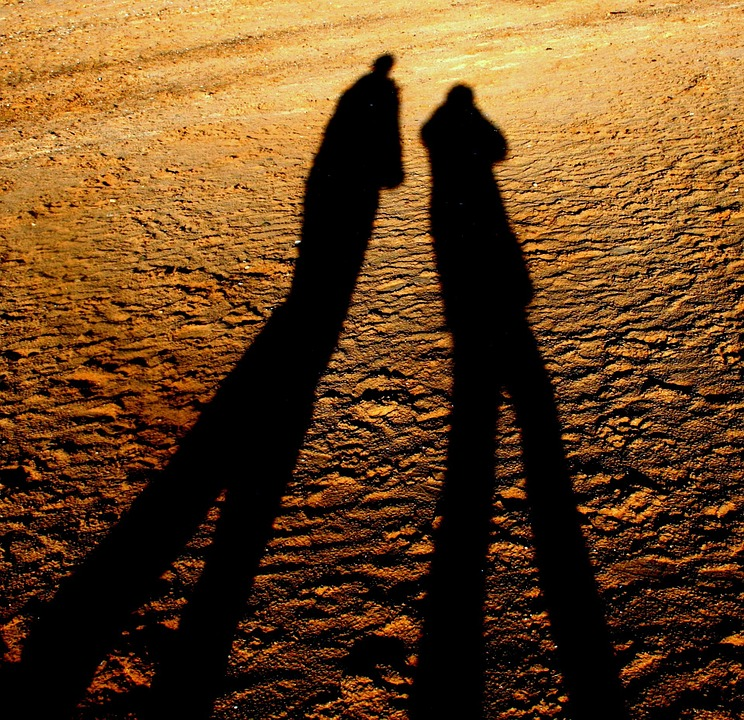
\includegraphics[width=0.7\linewidth]{images/schatten_personen.jpg}
	\captionof{figure}[schatten-relativ]{Schatten zweier Personen (\cite{PixaXX})}
	\label{fig:schatten-relativ}
\end{minipage}
\vspace{1em} 

Abbildung \ref{fig:schatten-relativ} zeigt diesen Sachverhalt. Anhand der Schatten der beiden Personen, lässt sich schließen, dass die rechte Person vermutlich kleiner ist als die linke Person.\\
\\
Außerdem lässt sich durch die Ausrichtung der Schatten auf auf die 'räumliche Beschaffenheit' schließen, wie Abbildung \ref{fig:schatten-raum} zeigt.\footcite[Vgl.]{heidXX} Abbhängig davon, wie die Schatten fallen, ändert sich die Perspektive auf das Objekt.\\

\vspace{1em}
\begin{minipage}{\linewidth}
	\centering
	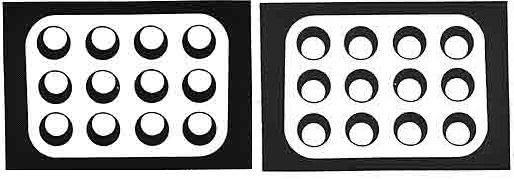
\includegraphics[width=0.7\linewidth]{images/schatten01.jpg}
	\captionof{figure}[schatten-raum]{Räumliche Beschaffenheit (\cite{heidXX})}
	\label{fig:schatten-raum}
\end{minipage}
\vspace{1em} 

\subsection{Vertraute Größe}
...

\subsection{Relative Helligkeit und perspektivische Unschärfe}
...

\subsection{Texturdichte-Gradient}
...

\subsection{Lineare Perspektive}
...

\subsection{Relative Höhe / Lage zum Horizont}
...

\subsection{Abgrenzung zu binokularen Tiefenkriterien}
...

\subsection{Anwendungsbereiche im Allgemeinen}
...

\subsection{Reale Beispiele}
...

\section{Konzeption}
...

\section{Umsetzung}
...

\section{Zusammenfassung}
...